\documentclass[a4paper]{article} % canviar a report!!!!!!!!!!!!!

\usepackage{amsmath}
\usepackage{graphicx}

\usepackage{anyfontsize}

\usepackage{fancyhdr}
\pagestyle{fancy}

\usepackage{titlesec}
\titleformat{\chapter}[block]
{\normalfont\huge\bfseries}{\thechapter.}{1em}{\Huge}
\titlespacing*{\chapter}{0pt}{-19pt}{19pt}


\titleformat*{\subsubsection}{\normalsize\bfseries}


\usepackage[nottoc,numbib]{tocbibind}

\usepackage{eurosym}
\usepackage{multirow}

%\renewcommand{\familydefault}{\sfdefault} % sans serif default

%\usepackage[none]{hyphenat}
\usepackage{hyphenat}

\usepackage{float}

\usepackage[catalan]{babel}

\usepackage[export]{adjustbox}[2011/08/13]

\usepackage[utf8]{inputenc}
\usepackage[titles]{tocloft}

\setcounter{tocdepth}{1} % Show sections
\setcounter{tocdepth}{2} % + subsections
%\setcounter{tocdepth}{3} % + subsubsections
%\setcounter{tocdepth}{4} % + paragraphs
%\setcounter{tocdepth}{5} % + subparagraphs

% To control the numeration of figures and tables
\usepackage{chngcntr}
%\counterwithin{figure}{section}
%\counterwithin{table}{section}


\title{Aplicació del \textit{Material Point Method (MPM)} a la deformació d'objectes}

\author{Martín Garcia, Pol}
\date{\parbox{\linewidth}{\centering%
		2019, Quadrimestre de tardor\endgraf\bigskip
		Director: Susín Sánchez, Toni\endgraf \medskip
		Especialitat Computació \endgraf
}}

\lhead{
\includegraphics[width=5cm]{images/logo-fib.png}}
\rhead{\fontsize{5}{6}\selectfont{\textbf{\textit{MPM} a la deformació d'objectes} \\
			Lliurable final GEP\\}}
		
	
\renewcommand{\figurename}{Imatge}

	
\widowpenalties 1 10000 % do not cut paragraphs
\raggedbottom

\setlength{\parindent}{0em}
\setlength{\parskip}{0.4em}

\usepackage[hidelinks]{hyperref}
\usepackage{url}



\begin{document}
	\pagenumbering{gobble}

\begin{titlepage}
	
	\begin{center}


	
		
\includegraphics[width=12cm]{images/logo-fib.png} % also works with logo.pdf
	\vfill
	
	\Huge
	\textbf{Aplicació del \textit{Material Point Method (MPM)} a la deformació d'objectes}  
	
	\vspace{0.5cm}
	\LARGE
	Lliurable final GEP

	\vspace{1.5cm}
	
	\textbf{Martín Garcia, Pol}

	\vfill
	
	Treball de final de grau d'Enginyeria informàtica
	
	\vspace{0.8cm}
	
	\Large
	Especialitat de Computació \\
	Tardor 2019 \\
	\vspace{0.5cm}
\textbf{Director: Susín Sánchez, Toni}
	\end{center}
\end{titlepage}


	\newpage
	

	\renewcommand{\contentsname}{Índex}
	\renewcommand{\cftsecfont}{\normalfont\bfseries}
	
	\tableofcontents
	\newpage
	

	% S'HA D'EDITAR LA PAGINA MANUALMENT SEMPRE

	\listoffigures
	\listoftables
\newpage
	\pagenumbering{arabic}	
	\setcounter{page}{3}
	\iffalse
	\chapter{Introducció}
	Aquest treball de fi de grau ha estat centrat en la simulació de fluids, una temàtica molt àmplia que tot i que conceptualment sembla trivial, és molt complexa. Molts detalls i decisions s'han de tenir en compte a l'hora d'implementar un simulador d'aquestes característiques, com la representació del fluid, si aquest és compressible, elàstic, interactiu amb col·lisions, etc. \par
	Per a poder presentar el treball correctament, aquest document també serveix com a introducció a la simulació de fluids sense assumir coneixements previs en aquest aspecte, i des del punt de vista d'un enginyer informàtic.\par
	I finalment també es busca mostrar com materials sòlids-elàstics es poden representar i simular com a fluids.
\fi
	\section{Context}
	La simulació de fluids, o dinàmiques de fluids computacionals (\textit{CFD's}), és una disciplina que, mitjançant tècniques d'anàlisi numèrica, busca resoldre problemes que impliquen d'alguna manera un tipus de fluctuació o interacció amb fluids. \par
	La base de qualsevol simulador de fluids són les equacions de Navier-Stokes, que descriuen la mecànica d'aquests; però necessitem molt més que les equacions per a poder implementar aquest programa, doncs també són necessaris coneixements de software i hardware per a una implementació eficient, tècniques de gràfics per computador per a una adequada visualització, i coneixements matemàtics d'àlgebra lineal que ja s'han vist durant l'educació oferida per la Facultat d'Informàtica de Barcelona, sobretot en la branca de computació. Tot i això, l'abast del projecte ens obliga a sortir de l'àmbit de coneixements d'un enginyer informàtic, i integrar múltiples conceptes matemàtics de diferents caires, que seran explicats degudament. \par
	Amb l'objectiu de poder sortejar aquest inconvenient, doncs els coneixements que he mencionat anteriorment a la FIB s'instrueixen en assignatures de màster impartides per professors d'altres facultats, el projecte s'està duent a terme sota la supervisió d'un professor del departament de matemàtiques de la UPC, cobrint d'aquesta manera les mancances de coneixement d'un enginyer informàtic en aquest camp.\par
	En el nostre cas les matemàtiques ens ajudaran a definir el comportament i les limitacions del nostre simulador, que a partir d'ara anomenarem també \textit{solver}, per a poder configurar-lo amb coneixement a posteriori, i sempre ser conscients de l'estat del sistema que s'està processant. \par
	És a dir, el problema a resoldre, simplificadament, consisteix a computar milers d'interaccions de forces, que segueixen un model físic o matemàtic concret, de manera molt eficient gràcies a certes aproximacions i generalitzacions, amb l'objectiu final d'obtenir una simulació visualment realista.
	
	\subsection{Conceptes bàsics}
	Abans d'entrar en detalls, hi ha uns coneixements bàsics que s'han de tenir en compte degut a l'àmplia projecció dels simuladors de fluids.
	\subsubsection[Tipus de solvers]{Tipus de solvers}
	Podem diferenciar els tipus de \textit{solvers} en 3 subgrups, que varien intrínsecament en el mateix concepte de la representació del fluid i els algorismes emprats. Aquesta representació marcarà la manera d'interactuar i tractar el fluid tant amb si mateix, com amb cossos externs.
	
	\paragraph[Graella]{\quad Solvers en Graella} Podem representar el fluid en un instant de temps concret com a una magnitud en un punt d'una graella, identificant la quantitat de fluid en aquella posició en un moment concret; per altra banda, cada cel·la de la graella té alguna representació de direcció i magnitud de moviment del fluid, per a poder computar el desplaçament d'aquest. \par
	A més a més, podem emmagatzemar altra informació a cada posició de la graella, o usar les dades ja guardades per a processar l'estat del sistema en un instant de temps posterior, tenint en compte que a cada cel·la només hi pot haver una quantitat màxima de fluid (volum màxim) perquè no sigui un fluid comprimible, i així provocar una dissipació d'aquest i el consegüent moviment.\par
	En conjunt, creem un espai acotat per les dimensions de la graella on el fluid es mou de manera quantitativa a través de les diferents cel·les, d'acord amb la mateixa informació d'aquestes. \par
	Aquesta representació es coneix com a simulador Eulerià.
	
	\paragraph[Partícules]{\quad Solvers de Partícules} Podem representar un petit volum de fluid com a una partícula en una posició determinada en un instant de temps, de manera que sempre representa la mateixa quantitat de fluid, i a més guardem tota la informació de moviment (força, velocitat, ...) a un nivell molt concret representat per la mateixa partícula. \par
	És important entendre que les partícules no representen el fluid a escala de molècules o àtoms, sinó que cada partícula representa una porció contínua del material o fluid, o un subconjunt del domini físic a simular.
	\par
	Aquesta representació permet, per exemple, barrejar dos fluids mantenint alhora les seves propietats separades, o simular interaccions entre partícules o sòlids externs amb un major nivell de detall.
	També cal dir, que aquest mètode dificulta la tasca de mantenir un volum constant del fluid, i sobretot necessita calcular interaccions entre totes les partícules, còmput que resulta molt costós. \par
	Els simuladors de partícules són coneguts com a Lagrangians.
	
	\paragraph[Híbrids]{\quad Solvers Híbrids} Si mesclem els dos conceptes anteriors, obtenim un simulador que, podem dir, rep el millor dels dos mètodes.\par
	Per una banda, es representa el fluid com partícules en cada instant de temps amb totes les seves propietats; i per altra banda el còmput d'interaccions entre aquestes el gestionem mitjançant una graella (la qual defineix l'espai del sistema) a on traspassem les característiques de les partícules en determinades zones, de manera que la computació de col·lisions i/o interaccions és molt més eficient i acotada.
	
	\subsubsection[MPM]{Material Point Method}
	Un dels mètodes que ara ha ressorgit per a la simulació de fluids és el conegut \textit{Material Point Method}, proposat per Sulsky \cite{Sulsky1995}, basat en partícules Lagrangianes i una graella Euleriana de rerefons. Aquest mètode és usat donat la seva alta eficiència de còmput, i la possibilitat de detallar la seva precisió amb la mida de la graella. \par
	Aquesta tècnica intenta emmagatzemar les dades de les partícules interpolades en les cel·les més properes, du a terme els càlculs en la graella, i finalment es fa la interpolació de manera inversa i es produeix el desplaçament de la partícula. \par
	Tot i això \textit{MPM} té alguns problemes, ja que per culpa de la simplificació que es produeix a la graella no som capaços de representar velocitats discontínues, o col·lisions molt concretes amb objectes de menor resolució de la graella. 
	
	
	\subsubsection{Propietats del fluid} 
	Un fluid sempre ha de tenir representades, en alguna determinada estructura o directament en l'algorisme, un seguit de propietats que el defineixen i n'especifiquen el comportament. Cal dir, que només és necessari usar aquelles propietats que el nostre model té en compte.
	\paragraph{\quad Volum} La quantitat de fluid que volem simular té un impacte directe en el nostre \textit{solver}, i depenent de la representació del fluid aquest concepte afectarà de manera diferent; per exemple, en simuladors de graella, massa fluid pot saturar el model; i en simuladors de partícules hem de controlar la proximitat entre partícules perquè aquesta defineix el volum.
	\paragraph{\quad Massa} Depenent del model a implementar, ens pot interessar la massa del fluid (representada, per exemple, en densitat) per a tractar la interacció amb forces externes (col·lisions o gravetat).
	\paragraph{Elasticitat} L'elasticitat és l'habilitat d'un cos o material de recuperar la seva forma original després d'una deformació, i alhora resistir-se a aquestes forces de deformació. Es descriu amb el model i la llei de Hook, que estipula que la força de retorn és proporcional a l'extensió de la deformació.
	\paragraph{\quad Viscositat} Molt semblant a l'elasticitat, la viscositat d'un fluid és la resistència que té a deformar-se o, informalment, a escampar-se. Es mesura en pascals per segon ($\frac{Pa}{s}$ o $\frac{kg}{m \cdot s}$) i es representa amb $\mu$ o $\eta$. És molt comú representar aquesta magnitud en relació amb la densitat $\rho$ de manera $\nu = \frac{\mu}{\rho}$ per a simplificar expressions.
	\paragraph{\quad Plasticitat} Si l'elasticitat defineix la possible deformació d'un cos, la plasticitat marca el punt de no retorn d'una deformació, en què les forces que busquen el retorn de l'objecte a l'estat original són permanentment degradades, de manera que part de la deformació es torna permanent. La idea de modelar aquesta característica, i el pioner treball de Terzopoulos et al. \cite{Terzopoulos:1988:MID:378456.378522} el 1988, ha fet que la simulació de materials topològicament canviants sigui una popular àrea d'estudi a gràfics per computador, on es poden tractar fets com la fractura (límit de la plasticitat), i el tallament d'objectes deformables. Totes aquestes interaccions s'anomenen inelàstiques.
	\paragraph{\quad Viscoelasticitat} Propietat dels materials que són viscosos i elàstics alhora en el moment de deformar-se. La viscositat fa que, a mesura que el temps avança, el material sofreix una tensió que li provoca una certa deformació, de manera que tota deformació elàstica sempre comporta una pèrdua d'energia a causa de la viscositat, produint una deformació plàstica.
	
	
	\subsection{Formulació del problema}
	Podríem considerar que hi ha dos tipus de simulacions: les que tenen com a objectiu emular la realitat, i les que busquen obtenir una animació visualment realista.\par
	Les simulacions que imiten la realitat tendeixen a requerir moltíssima precisió i algorismes poc optimitzables, les quals acostumen a necessitar ser processades en un supercomputador per obtenir resultats adequats en un temps raonable. \par
	Per altra banda, la simulació amb objectius només visuals (com és el nostre cas) intenta ser ràpida, visualment realista i, sobretot, configurable per a poder triar quins resultats es volen aconseguir. Encara que no s'intenti emular la realitat al cent per cent, és important imitar-la al màxim acceptant generalitzacions i truncaments per a accelerar la velocitat de computació; depenent de la situació podríem simplificar el model el suficient per arribar a tenir una simulació en temps real.\par
	A causa del fet que es busca trobar una fidel i ràpida aproximació a la realitat, no existeix una solució analítica (ni general ni específica) per a produir aquestes simulacions. També s'ha de tenir en compte quina és la versatilitat de la simulació, perquè el mateix algorisme implementat limitarà les propietats del fluid o sòlid. Finalment també hi ha la possibilitat, i el problema, de fer interaccionar el fluid a simular amb algun cos extern (tant en moviment com immòbil) i la transmissió de forces entre aquests. \par
	Així doncs, aquest treball pretén estudiar com plantejar solucions per a implementar les qüestions anteriors, i alhora aplicar-les per a conèixer les limitacions i habilitats de cadascuna, en un determinat sistema; i també servir com a base introductòria a aquesta temàtica tan dispersa i tècnica a qualsevol lector.
	
	\subsection{Actors implicats}
	En aquesta secció es definiran els actors implicats, de manera directa i indirecta, en el projecte.
	\paragraph{\quad Director} Figura essencial pel correcte desenvolupament del projecte, i màxim responsable en la guia i consell al desenvolupador del treball. La seva acció és clau per determinar errors en el projecte, tant de tipus proposicional com executius. En aquest cas el director és Toni Susín Sánchez, del departament de Matemàtiques Aplicades de la UPC, i cap del \textit{Dynamic Simulation Lab} inclòs en el grup de recerca ViRVIG.
	\paragraph{\quad Desenvolupador} La persona a càrrec de dur a terme la recerca, documentació i implementació del software requerit, així com de redactar la memòria del projecte sota la guia del director. També recau sobre aquest actor la gestió del projecte, i és en última instància la persona responsable de complir amb els terminis del treball. Aquest rol recau sobre Pol Martín Garcia, alumne de la FIB de la branca de computació.
	\paragraph{\quad Entorn} El centre de treball ViRVIG (Visualització, Realitat Virtual i Interacció Gràfica) ha facilitat un entorn de treball per a poder usar i provar el projecte amb la potència de còmput necessària, i aprovisionat d'un clima de treball per al correcte desenvolupament del projecte.
	\paragraph{\quad Usuaris} Aquest treball busca crear una dissertació i ampliació dels simuladors d'avui dia, i com a tal no tindrà usuaris directes. Qualsevol avanç en \textit{solvers} de tota mena, però, té un impacte parcial en la investigació i implementació de noves tècniques d'animació; com per exemple en efectes especials de pel·lícules, com a \textit{Big Hero 6}, \textit{Zootopia}, o inclús \textit{Frozen} de Disney \cite{Stomakhin} per a simular la neu.
	\paragraph{\quad Beneficiaris} Perquè aquest projecte no crearà un producte, com s'ha dit abans, tampoc hi ha beneficiaris directes. No obstant això, altres estudiants d'enginyeria informàtica o matemàtiques poden trobar aquest projecte interessant com a base d'aprenentatge, i usar-lo com a punt de partida per a futurs projectes centrats en l'àmbit de simulació de fluids en \textit{MPM}.
	
	\section{Justificació}
	Aquesta temàtica és una àmplia àrea d'estudi des de fa diverses dècades, que s'ha anat dividint en múltiples tècniques i cada branca d'estudi va aprofundint en paral·lel de la resta.
	\par
	En aquest treball estudiarem i implementarem un \textit{solver} \textit{MPM}, que neix de la generalització de \textit{Particle in Cell} (PIC) i \textit{Fluid Implicit Particle Method} (FLIP) \cite{Sulsky1995}. Hi ha hagut molt nombrosos i extensos treballs de FLIP en els darrers anys \cite{Bridson2018,Zhu2005}, mentre que \textit{MPM} ha sigut realment introduït i començat a estudiar recentment perquè, al contrari que FLIP, aquest pot tractar amb fluids i sòlids comprimibles.
	\par
	D'aquesta manera, \textit{MPM} s'està començant a estudiar i a usar per a simular diferents tipus d'interaccions innovadores. Com s'ha dit abans, ressalta la simulació de neu de Disney \cite{Stomakhin} o l'interacció entre o amb múltiples materials deformables\cite{Hegemann2013}, per posar alguns exemples. Es pot trobar més informació dels treballs en \textit{MPM} a \cite{Jiang2016}.
	\par
	Just molt recentment ha sorgit una nova tècnica per a resoldre \textit{MPM}, anomenada \textit{MLS-MPM} (\textit{Moving Least Squares Material Point Method})\cite{hu2018mlsmpmcpic} que, generalment, busca millors aproximacions a la graella gràcies a una \textit{B-spline}\footnote{Funció corba; és detallarà en futurs apartats.} calibrada amb \textit{MLS}.
	\par
	D'aquesta manera, i amb base als nous desenvolupaments de Yuanming Hu et. al. a \cite{hu2018mlsmpmcpic} i usant com a base \cite{Hu} dels mateixos autors, estudiarem aquesta tècnica i possibles diferents interpretacions del model. És a dir: adaptarem la solució de Yuanming a unes necessitats personals i investigarem com reacciona el sistema a unes noves condicions.
	\par 
	Aquest projecte sorgeix de la curiositat personal del desenvolupador sobre aquest tipus de software, la teoria que hi ha al darrere, i l'atractiu dels resultats obtinguts. Una temàtica que, personalment es considera, no té la suficient visibilitat per la importància i complexitat que té. Per tant, amb aquest treball s'espera poder donar a conèixer més aquests programes i les seves aplicacions.
	\par
	Finalment, cal dir que existeix molt poc material, tant a la literatura com a la xarxa, que serveixi d'introducció a aquest camp, sobretot des del punt de vista informàtic. D'aquesta manera s'espera que aquest document pugui ser usat com a preliminar d'aprenentatge en l'àmbit de simuladors de fluids, aprofitant la simplificada versió de \textit{MLS-MPM}, molt més senzilla i òptima que la competència, aprofundint en el trasllat del simulador a 3D per a simulacions visualment realistes.
	
	\section{Abast}
	En aquesta secció definirem quines són les fites del projecte, i la seva estructura progressiva.
	\subsection{Objectius}
	\paragraph{\quad Aprenentatge de nous conceptes} Donat que el treball requereix de coneixements allunyats dels adquirits en una enginyeria informàtica, cal una cerca intensiva d'informació i aprenentatge de mètodes numèrics, càlcul, i àlgebra lineal. Tots aquests conceptes són necessaris per entendre els diferents models d'objectes i simuladors a implementar. \par
	En concret, existeixen alguns subtemes que mereixen una menció especial com a subobjectius:
	
	\begin{itemize}
		\item \textbf{Les equacions de Navier-Stokes} Aplicant la segona llei de Newton al moviment del fluid, amb algunes assumpcions de les forces internes (anomenades estrès), s'obtenen les equacions de Navier-Stokes; conegudes per la seva complexitat, que ja de per si obren una interessant àrea d'estudi de possibles implicacions i aplicacions.
		\par
		És important entendre aquestes equacions, i saber interpretar-les, doncs descriuran el nostre sistema i són la base de qualsevol \textit{solver}.
	\item \textbf{Càlcul vectorial} Fins a un cert nivell, és important i necessari conèixer diferenciació i integració de camps vectorials, doncs tractarem amb camps de partícules en aquest projecte.
	\item \textbf{Tècniques de solvers} Finalment, amb els coneixements teòrics necessaris, s'ha d'aprendre el funcionament intern i els models que permeten simular els diferents tipus de \textit{solvers} creats, en concret el de \textit{MLS-MPM} \cite{hu2018mlsmpmcpic}.
	\end{itemize}
	\paragraph{\quad Implementació d'un solver bidimensional} Per a una primera versió, serà implementat un simulador de fluids de partícules bidimensional, seguint\cite{Hu,hu2018mlsmpmcpic} i programant la base de tot el projecte a una escala menor, per a fer proves i trobar errors. La idea és usar aquesta primera fase com a indicador, i prendre decisions d'acord amb els resultats obtinguts per a millorar el resultat final, i evitar errades. \par
	L'objectiu d'aquesta etapa és el refinament de l'entorn de treball per a una posterior fase molt més complexa, i d'aquesta manera poder evitar nombrosos possibles errors, estudiar inconvenients que puguin aparèixer i, sobretot, com a guia d'aprenentatge progressiu de manera simplificada. 
	
	\paragraph{\quad Millora del solver a la tercera dimensió} El canvi de dimensió és un salt difícil, i essencial en aquest projecte, doncs tot simulador gràfic per a resultats realistes requereix aquesta tercera dimensió. Serà necessari redimensionar la interfície gràfica, les estructures de dades, i el mateix algorisme.
	\par
	A partir d'aquesta fita, és quan s'inicien els tests i objectius secundaris.
	
	\subsubsection{Objectius secundaris} En la mesura del possible, s'intentarà dur a terme els següents objectius, que no són necessaris per al correcte desenvolupament del projecte, però el completen i ajuden a veure com tractar i solucionar altres problemes inherents en qualsevol sistema programat.
	\paragraph[Interacció viscoelàstica]{\qquad Interacció entre diversos materials viscoelàstics diferents} Afegir suport per a poder mantenir en el simulador alhora diversos fluids de diferents característiques cadascun.
	\paragraph[Sistema de físiques]{\qquad Sistema de físiques} Implementar un sistema d'interacció de cossos sòlids en moviment amb el \textit{solver}, per aconseguir simular col·lisions amb un o diversos elements externs al simulador; com per exemple una roda amb sorra.
	\paragraph[Eficiència]{\qquad Eficiència} Sobretot en el \textit{solver} tridimensional, l'eficiència i velocitat del programa és un problema, ja que aproximadament el còmput de cada fotograma serà major a un minut segons els articles de \textit{MPM} \cite{hu2018mlsmpmcpic}; per tant sempre que es pugui s'ha d'implementar el simulador sent conscients de l'arquitectura i de l'eficiència del codi.
	\paragraph[Paral·lelisme]{\qquad  Paral·lelisme} Aconseguir que el codi funcioni de manera paral·lela pot suposar un increment de la velocitat de computació molt important. Així doncs, qualsevol oportunitat de paral·lelitzar el codi s'haurà d'aprofitar.
	
	
	\subsection{Requisits}
	Podem separar els requisits del software a implementar en funcionals, i no funcionals. Els primers representen funcionalitats específiques que el nostre sistema haurà de complir, i el segon especifica criteris per jutjar els comportaments específics d'aquest.
	
	\subsubsection{Requisits funcionals}
	\paragraph{\quad Simulació d'un sistema personalitzable} Amb modificació del nombre, tipus, i posició de les partícules; canvi del medi (gravetat, mida de la graella, etc). Cal valorar si han de ser paràmetres modificables entre execucions, o constants en el codi.
	\paragraph{\quad Exportació de la simulació} Exportació dels fotogrames produïts pel \textit{solver}, o bé en arxius binaris per al seu posterior tractament, o bé en imatges \textit{PNG} (\textit{Portable Network Graphics}).
 	\paragraph{\quad Simulació d'objectes viscoelàstics} Importació de models de triangles, i simular-ne el comportament en unes condicions especificades com a materials elàstics o viscoelàstics.
	
	\subsubsection{Requisits no funcionals}
	\paragraph{\quad Velocitat de computació} La velocitat del còmput ha d'estar justificada i ser adient; ha de ser linealment dependent del nombre de partícules o a la mida de la graella.
	\paragraph{\quad Estabilitat de la simulació} Les solucions del \textit{solver} han de ser estables, i no descontrolar-se; en cas de ser impossible evitar la inestabilitat, aquest fet estarà documentat i estudiat, marcant els límits del simulador.
	
	
	\subsection{Obstacles i riscos}
	Per evitar imprevistos en el transcurs del projecte, analitzarem els obstacles que poden sorgir durant aquest procediment i, sobretot, com minimitzar el seu impacte.
	\subsubsection{Errors en el codi}
	És inevitable cometre petits errors en la implementació d'un software, que a vegades poden passar desapercebuts, i altres vegades poden trencar totalment el programa.\par
	Donat que un simulador no pot ser testejat amb jocs de proves, serà necessari provar manualment cada nova característica afegida, i comprovar que totes les anteriors propietats segueixen funcionant adequadament. D'aquesta manera podrem minimitzar els riscos de perpetuar un error durant les diverses versions del software.
	\subsubsection{Problemes o insuficiència de hardware}
	Els ordinadors poden tenir problemes, els discos poden fallar, la memòria RAM pot deixar de funcionar, els arxius es poden corrompre, etc. Aquestes situacions suposen una pèrdua de temps important a curt termini per a reparar el hardware espatllat i recuperar les dades perdudes, en el no tan improbable cas de que succeeixin. \par
	Per evitar l'impacte d'aquest problema en la mesura de tot el possible, el projecte i la memòria d'aquest es guardaran per versions en un repositori a la xarxa, més concretament a \textit{GitHub}. A més a més, la memòria es guardarà en paral·lel al \textit{OneDrive} de Microsoft.
	\par
	Per altra banda, durant les etapes més avançades del projecte el temps de simulació es veurà incrementat quantitativament, cosa que provocarà que per provar els canvis siguin necessàries hores. \par
	Per a evitar perdre temps sense avançar adequadament, els tests (en forma d'execucions arbitràries del programa) es deixaran executant en una màquina diferent de la que es treballa, amb molta més potencia (com un dels ordinadors del ViRVIG) per obtenir els resultats tan aviat com sigui possible, sense entorpir el desenvolupament.
	\subsubsection{Errors de comprensió dels models matemàtics}
	A causa de la complexitat de les matemàtiques que hi ha darrere d'aquest projecte, i al fet que aquest és conceptualitza des del punt de vista informàtic, és possible errar en l'enteniment de nombrosos conceptes tècnics en, per exemple, els models elàstics dels objectes, el procediment del simulador, o en simples formalismes d'expressivitat matemàtica. 
	\subsubsection{Problemes temporals}
	Les limitacions temporals són inherents a tot projecte de fi de grau, i aquest no n'és una excepció. Si hi ha una mala gestió del temps, o algun tipus d'imprevist, podem trobar-nos amb la impossibilitat de complir tots els requisits i objectius del treball a temps. \par
	Per a aquest motiu és important escollir i seguir una metodologia, creant una planificació per a dur a terme el projecte. D'aquesta manera podem ser molt més conscients de l'avenç que s'està fent, i de ser necessari poder realitzar a temps modificacions a l'abast del mateix.
	
	\section{Metodologia i rigor}
	En qualsevol projecte de mínima magnitud, s'ha de triar i adherir-se a un sistema organitzatiu concret. D'aquesta manera podem tenir una visió molt més acurada del treball, i mantenir un ordre en aquest; a més de tenir sempre un procediment a seguir en cas de qualsevol inconvenient.
	\subsection{Metodologia}
	La metodologia emprada en el projecte per a la seva organització i concepció és la \textit{Kanban} \cite{Anderson2010}. Aquesta és una metodologia àgil molt semblant a \textit{Scrum}, però dissenyada per a mantenir un flux constant de resultats evitant discretitzar el projecte en \textit{sprints}. Aquest mètode aporta molta flexibilitat i permet focalitzar el treball en només el que es considera essencial. Podem observar una sintesi a la figura \ref{fig:kanban}
	\par
	\begin{figure}[h]
		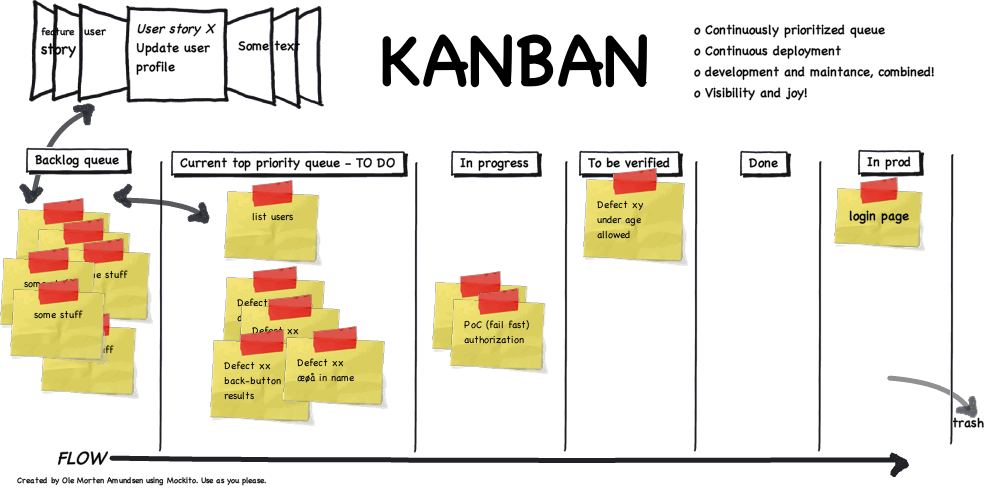
\includegraphics[width=\linewidth]{images/kanban_illustration.png}
		\caption[\textit{Metodologia Kanban}]{\textit{\small Metodologia Kanban}. Extreta de \url{https://olemortenamundsen.files.wordpress.com/2010/03/kanban_illustration.png} [Octubre 2019]}
		\label{fig:kanban}
	\end{figure}

	La principal idea darrere d'aquest mètode és mantenir sempre alguna tasca en procés, de manera que quan s'ha acabat quelcom, la següent tasca de més prioritat entra en acció. A més a més, s'ha d'evitar mantenir més d'una tasca en procés alhora, limitant la quantitat de \textit{work in progress} al mínim, i centrar-se en el més important en aquell moment.
	\par
	En cas de tenir qualsevol inconvenient, aquesta metodologia és molt responsiva als canvis i ens permet, ràpidament, corregir qualsevol aspecte mancant alhora que es valora la seva prioritat amb el director del projecte.
	
	\subsection{Eines de seguiment}
	Per al correcte seguiment del projecte, el seu estat i les seves versions, s'usen diverses eines. Primerament és important tenir una visió global del que es porta fet, i el que queda per fer; per a això s'usa el mètode de \textit{Bullet Journaling} per a ser conscients en tot moment de l'estat del projecte, a un nivell personal. \par
	A escala de codi, un historial de versions, organitzat adequadament per funcionalitats, és emmagatzemat a \textit{GitHub} juntament amb les diverses versions de la memòria del projecte. Amb aquesta eina podem tenir una visió ordenada del procés evolutiu del treball, veient les funcionalitats per separat.\par
	Finalment, també es duran a terme reunions periòdiques amb el director on es revisaran, entre altres coses, els avanços fets des de l'última reunió, l'estat del projecte, i dubtes i qüestions sorgides. Donada la naturalesa del projecte, en aquestes reunions es duran a terme explicacions teòriques de conceptes no vistos a la FIB per al correcte desenvolupament del projecte.
	\par
	En cas de sorgir problemes o imprevistos, es contactarà amb el director i, de ser necessari, es crearà un pla de contingència o una ruta a seguir per a solucionar qualsevol inconvenient.
	 

	\section{Planificació temporal}
	Aquest projecte es realitzarà en el marc temporal d'un quadrimestre, i en les següents pàgines es fa una planificació en tasques i una estimació de la durada d'aquestes.\par 
	Ja que el desenvolupament del projecte no és una activitat a temps complert, s'estima un mínim de 14 hores de treball setmanal en el mateix; però s'espera una mitjana de 25 hores d'involucració a la setmana. \par 
	Concretament, el projecte s'inicia a mitjans de juliol del 2019, amb la seva concepció, i s'allargarà fins a inicis de gener de l'any 2020 per al torn de lectures del mateix mes.
	
	\subsection{Descripció de tasques}
	A continuació es descriuen les diferents tasques a dur a terme en el projecte. Les tasques engloben fins a 4 subtasques, com a molt, per a poder oferir el màxim de detall en el mínim espai de document possible, les quals seran descrites i especificades. També s'afegeix la seva estimació temporal i les dependències entre elles. La taula \ref{table:resumTasques} mostra un resum d'aquesta secció a la pàgina \pageref{table:resumTasques}.
	\subsubsection{Base del projecte i entorn de treball}
	La primera tasca del projecte consisteix en la creació de les eines més bàsiques i elementals, i la familiarització amb aquestes, que seran necessàries per a acompanyar la implementació del \textit{solver}. També es codificarà una base adaptable per a interactuar amb el simulador en el futur.\par 
	
	Les eines a programar consisteixen en, usant la llibreria gràfica \textit{OpenGL} \cite{SiliconGraphics2013}, un visualitzador per pantalla de partícules per a veure en temps real els resultats; i seguidament també serà necessari implementar una eina per exportar els fotogrames en imatges, usant la llibreria \textit{open source stb\_image} \cite{stb}. 

	\paragraph{\quad Previsió temporal} 20 hores per al desenvolupament del visualitzador i la base del projecte, perquè han d'anar acoblades i requereixen certa planificació. 5 hores per a l'exportador d'imatges, ja que no és una eina complexa i no és innovadora, però es requereix prendre decisions sobre el format d'imatge a exportar.
	\paragraph{\quad Dependències} Aquesta primera tasca no té cap dependència, més enllà del fet que abans de poder implementar quelcom, un s'ha de familiaritzar amb el concepte.
	\subsubsection{Simulador de partícules simple}
	Fase que té com a objectiu principal l'aprenentatge del funcionament dels simuladors \textit{MLS-MPM}, implementant la seva versió més simple a sobre de la base creada a l'anterior etapa. \par 
	Aquest primer \textit{solver} serà molt semblant al codi de \textit{2D-MPM} en 88 línies de \cite{hu2018mlsmpmcpic}, però portat al terreny del projecte.\par 
	És important denotar que aquesta fase està dividida en dos: primerament s'ha de dur a terme un aprenentatge exhaustiu de la nova temàtica, i posteriorment l'anomenada implementació. \par 
	Es finalitzarà comprovant que la tasca ha estat realitzada correctament, mitjançant tests manuals, i es corregiran tots els errors trobats i esperats.
	\paragraph{\quad Previsió temporal} A causa de la gran quantitat de continguts a estudiar, s'assignen 65 hores dedicades a l'aprenentatge, pràctica i assoliment de conceptes nous. Posteriorment, s'estimen 25 hores per a la implementació, i 10 hores extres per a dur a terme la validació i correcció d'errors.
	\paragraph{\quad Dependències} D'aquesta tasca, a l'estar dividida en dos, només una part té dependències. L'aprenentatge es pot dur a terme de forma lliure; però la implementació requereix aquest aprenentatge previ, i que ja existeixi una base programada.
	
	\subsubsection{Addició de model elàstic}
	De la mateixa manera que la fase anterior, aquesta està dividida en aprenentatge i implementació, però dels models elàstics a incorporar en el simulador. En concret s'estudiarà \textit{CPIC} desenvolupat a \cite{hu2018mlsmpmcpic}, basat en \cite{Jiang2016}, i la seva addició de \textit{fixed corotated model} afegint l'estrès a \textit{CPIC} \cite{Hu,Jiang2016}. \par
	Finalment, s'haurà de validar el funcionament dels models elàstics.
	\paragraph{\quad Previsió temporal} Perquè l'estudi de models elàstics és d'un nivell molt avançat, i d'una branca molt separada a la d'informàtica, s'estima unes 60 hores màximes per al seu aprenentatge; posteriorment pel seu disseny i implementació s'assignen 30 hores; més 8 hores de validació i correcció d'errors. Aquestes estimacions són degudes a la inestabilitat dels mètodes a implementar.
	\paragraph{\quad Dependències} Igual que a l'anterior tasca, en aquesta només la implementació de models elàstics requereix del seu aprenentatge i de l'existència d'un simulador de fluids de partícules.
	
	\subsubsection{Optimització i estudi 2D}
	Juntament amb el director, s'analitzarà el \textit{solver} actual i s'estudiarà quines zones requereixen alguna millora, o poden admetre optimitzacions interessants. També es discutirà sobre com plantejar-se la migració del simulador de dues dimensions a una tercera. \par
	Durant aquesta etapa també es veuran les oportunitats de paral·lelitzar el codi i millorar-ne la precisió del simulador, juntament amb la seva posterior implementació.\par
	En aquesta fase també incorporem l'estudi del simulador, juntament amb el perfeccionament dels paràmetres del mateix, i els diferents comportaments depenent de l'entrada.
	\paragraph{\quad Previsió temporal} S'estimen 30 hores de feina per a millorar i canviar fragments de codi necessaris per a una bona evolució. Per a implementar paral·lelisme s'assignen a part 15 hores a causa de la diferenciació de tipologia de problema que suposa.
	\paragraph{\quad Dependències} Per a poder dur a terme l'estudi, és necessari que el simulador estigui complet i funcional.
	\paragraph{\quad Recursos} En aquesta tasca, per a provar el paral·lelisme serà necessària una màquina amb diversos nuclis.
	
	\subsubsection{Primera documentació}
	L'inici de la documentació, planificació, definició de l'abast i anàlisi detallat de l'enfocament del projecte es du a terme en aquesta tasca, a la tercera part del desenvolupament del projecte, per a puntualitzar el procediment a seguir per al seu correcte desenvolupament. \par
	Tots aquests detalls es plasmaran en una memòria del projecte, efectuada en \textit{LaTex} \cite{latex}, adjunta a la documentació i experimentació duta a terme.\par
	És important puntualitzar el desenvolupament d'altres tasques en aquesta etapa com l'anàlisi de sostenibilitat, la planificació temporal, gestió econòmica i de riscos, i la metodologia del projecte.
	\paragraph{\quad Previsió temporal} S'estimen unes hores invertides en aquesta etapa majors que les desitjables, perquè també s'hauran d'aprendre conceptes nous i redactar alhora. S'usaran 35 hores dedicades a l'escriptura de documentació, i 20 a l'estudi, planificació i concepció dels temes a tractar. S'afegeixen 10 hores per a realitzar correccions i replanificar el necessari.
	\paragraph{\quad Dependències} La primera documentació no s'iniciarà fins que ja s'hagi tingut un tast en el desenvolupament del projecte, per a poder entendre'l bé i, en conseqüència ser capaços d'estimar i planificar el desenvolupament del mateix.
	
	\subsubsection{Millora a 3D}
	Aquesta etapa tracta íntegrament la translació del projecte a la nova dimensió, a discutir el procediment amb el director del projecte arribat el moment, doncs hi ha moltes maneres diferents d'aproximar aquest canvi depenent del desenvolupament del treball. \par
	De totes formes, podem enumerar les característiques que s'hauran de canviar concretament:
	\begin{itemize}
		\item Estructures de dades: s'ha d'incorporar la nova coordenada a emmagatzemar per la posició de les partícules, i modificar la graella perquè sigui tridimensional.
		\item Model elàstic: La matemàtica darrere el model requereix canvis importants per a poder funcionar.
		\item Algorisme: Per a adaptar els canvis anteriors, alguns retocs a l'algorisme s'hauran de fer.
		\item Visualitzador: S'ha d'idear alguna forma de poder visualitzar una zona de l'espai 3D de la simulació.
	\end{itemize}

	Un cop els canvis han sigut implementats, és necessari dur a terme una validació intensiva i exhaustiva d'aquestes modificacions, doncs no són trivials i requereixen molta especialització.
	\paragraph{\quad Previsió temporal} En aquesta etapa es dedicarà 30 hores a la implementació i gestió de canvis en el simulador; i posteriorment 30 hores més de validació de resultats, donat que es tracta d'una etapa molt delicada on la velocitat del sistema es reduirà, i la complexitat augmentarà.
	\paragraph{\quad Dependències} La millora a la tercera dimensió requereix de l'existència d'un \textit{solver} finalitzat en dues dimensions, optimitzat, i estudiat per a facilitar aquesta tasca.
	\paragraph{\quad Recursos} En aquesta tasca, és necessari el PC del \textit{ViRVIG} per a dur a terme la validació.
	
	\subsubsection{Estudi 3D}
	Amb el simulador correctament implementat, podem passar a l'etapa de documentació, estudi, i ajustament dels paràmetres del simulador. Durant aquesta fase es documentaran totes les modificacions finals dutes a terme durant el canvi a la tercera dimensió, i perfeccionar la configuració del \textit{solver} per a obtenir resultats adequats. \par
	Si es valora necessari, amb l'estudi efectuat s'implementaran i es provaran aquelles millores que siguin senzilles i directes, ja que la complexitat del disseny de modificacions en una dimensió extra, i la posterior validació d'aquestes, seria molt costosa.
	\paragraph{\quad Previsió temporal} S'assignen 10 hores de documentació de treball en la millora a 3D; 20 hores més d'estudi dels resultats i paràmetres del \textit{solver}, i 30 més de valoració, implementació i validació de millores.
	\paragraph{\quad Dependències} L'anàlisi del simulador tridimensional requereix de la correcta implementació d'aquest.
	\paragraph{\quad Recursos} Per a la validació serà necessari el PC del \textit{ViRVIG}, i aprofitar la seva potència.
	
	\subsubsection{Físiques}
	Si la planificació no és esbiaixada de manera important, es podrà dur a terme aquesta etapa. \par
	Diferenciant l'aprenentatge de la implementació, es busca arribar a codificar un sistema de col·lisions entre objectes externs al simulador i les partícules d'aquest, de manera que es puguin dur a terme animacions amb interaccions. \par
	Serà necessari, primer de tot, implementar un sistema de càrrega de models simples tridimensionals, i posteriorment un mecanisme d'interacció i transmissió de forces unidireccional (del model al simulador), com els mostrats a \cite{Ericson2005}. \par
	Serà necessari validar, estudiar i documentar adequadament aquesta etapa, doncs proporcionarà alguns dels resultats més interessants de tot el projecte.
	\paragraph{\quad Previsió temporal} S'estima un temps d'estudi de 20 hores; i un temps d'implementació de 30 hores al complet. S'ha d'afegir unes 20 hores de validació de resultats, i unes altres 10 per a codificar eines externes de càrrega i prova de models.
	\paragraph{\quad Dependències} Com que aquesta tasca està diferenciada en estudi i implementació, només la darrera requerirà l'aprenentatge de físiques i d'una codificació finalitzada d'un \textit{solver} 3D.
	
	\subsubsection{Documentació final}
	Finalitzant el projecte, s'ha de consolidar la documentació i la memòria d'acord amb el software creat, i tancat ja per a aquesta etapa. Aquí se sintetitzaran tots els resultats del programari, els estudis i descobertes interessants. \par
	Serà important generar exemples per a poder mostrar les funcionalitats dels resultats del treball, i per justificar les conclusions.\par
	Per últim s'hauria de tenir molt en compte la reunió de seguiment, que a ser possible es realitzarà ben entrada aquesta etapa, per a l'adequada finalització del projecte i la respectiva preparació de l'entrega final, la seva correcció, i la presentació final del treball de fi de grau.
	\paragraph{\quad Previsió temporal} S'assignen 60 hores de treball en la memòria i documentació final, dividides en 18 hores per documentar el programa, 30 hores per a redactar el document de tot el que no ha estat ja escrit, i 12 hores més de correcció d'errors i revisió. Finalment també s'han de tenir en compte unes 20 hores de preparació de la defensa final.
	\paragraph{\quad Dependències} En ser l'etapa final del projecte, dependrà de totes les fases anteriors.
	
	\subsection{Recursos Humans}
	En aquest projecte s'involucraran, en diferent mesura, les tasques pròpies d'un desenvolupador o programador, que s'encarregarà d'implementar el treball; un analista, per a avaluar tots els paràmetres i el comportament del \textit{solver} sota diferents condicions, intentant optimitzar al màxim possible aquest; un enginyer de tests, per a poder validar el simulador en qualsevol etapa; i un coordinador de projecte, per a poder planificar i gestionar tots els recursos, tant materials com temporals.
	\par
	Els Recursos Humans es troben assignats a la taula \ref{table:resumTasques}.
	\newpage
	\subsection{Taula resum}
	A continuació s'adjunta la taula \ref{table:resumTasques}, que mostra l'estimació d'hores de les múltiples tasques del projecte, així com les dependències entre elles. En cas de cascada de dependències, només s'indica l'últim prerequisit.
	\begin{table}[h!]
		\centering
		\hspace*{-0.5cm}
		\begin{tabular}{|| c || c | c | c c||}
			\hline
			\textbf{Id} & \textbf{Nom} & \textbf{RRHH} & \textbf{Hores} & \textbf{Dependències} \\ 
			\hline\hline
			1 & Creació de la base & Desenvolupador & 25 & no \\
			\hline
			2.1 & Aprenentatge \textit{solver} & Desenvolupador & 65 & no \\
			2.2 & Implementació \textit{solver} & Desenvolupador & 25 & 1, 2.1 \\
			2.3 & Validació \textit{solver} & Tester & 10 & 2.2 \\
			\hline
			3.1 & Aprenentatge models elàstics & Desenvolupador & 60 & no \\
			3.2 & Implementació models elàstics & Desenvolupador & 30 & 2.3, 3.1 \\
			3.3 & Validació models elàstics & Tester & 8 & 3.2 \\
			\hline
			4.1 & Estudi 2D & Analista & 30 & 3.3 \\
			4.2 & Paral·lelisme & Desenvolupador & 15 & 4.1 \\
			\hline
			5.1 & Documentació: planificació & Coordinador & 20 & 2.3 \\
			5.2 & Documentació: redacció & Coordinador & 35 & 2.3, 5.1 \\
			5.3 & Documentació: correcció & Coordinador & 10 & 5.2 \\
			\hline
			6.1 & 3D: migració & Desenvolupador & 30 & 4.2 \\
			6.2 & 3D: validació & Tester & 30 & 6.1 \\
			\hline
			7.1 & Estudi 3D & Analista & 20 & 6.2 \\
			7.2 & Documentació 3D  & Coordinador & 10 & 6.2 \\
			7.3 & Estudi 3D: millores i validació & Desenvolupador & 30 & 7.1 \\
			\hline
			8.1 & Aprenentatge físiques & Desenvolupador & 20 & no \\
			8.2 & Implementació físiques & Desenvolupador & 30 & 7.3, 8.1 \\
			8.3 & Validació físiques & Tester & 20 & 8.2 \\
			8.4 & Implementació eines & Desenvolupador & 10 & 8.1 \\
			\hline
			9.1 & Documentació programa & Desenvolupador & 18 & 8.3 \\
			9.2 & Redacció memòria & Coordinador & 30 & 9.1 \\
			9.3 & Revisió i correcció & Coordinador & 12 & 9.2 \\
			9.4 & Preparació defensa final & Coordinador & 20 & 9.3 \\
			\hline \hline
			- & Total & - & 613 & - \\
			\hline
		\end{tabular}
	\caption[\textit{Resum de tasques}]{\textit{\small Resum de tasques}. Elaboració pròpia}
	\label{table:resumTasques}
	\end{table}
	
	En comparació amb el diagrama de Gantt de la figura \ref{fig:Gantt}, de la pàgina \pageref{fig:Gantt}, i la nostra anàlisi, podem veure una diferència de 22 hores. Això és degut al fet que en el diagrama s'ha intentat afegir, de manera distribuïda, hores per a realitzar consultes i reunions amb el director en les diverses tasques, i també donant un marge de seguretat temporal.
	
	\newpage

	\begin{figure}[H]
	\subsection{Diagrama de Gantt}
		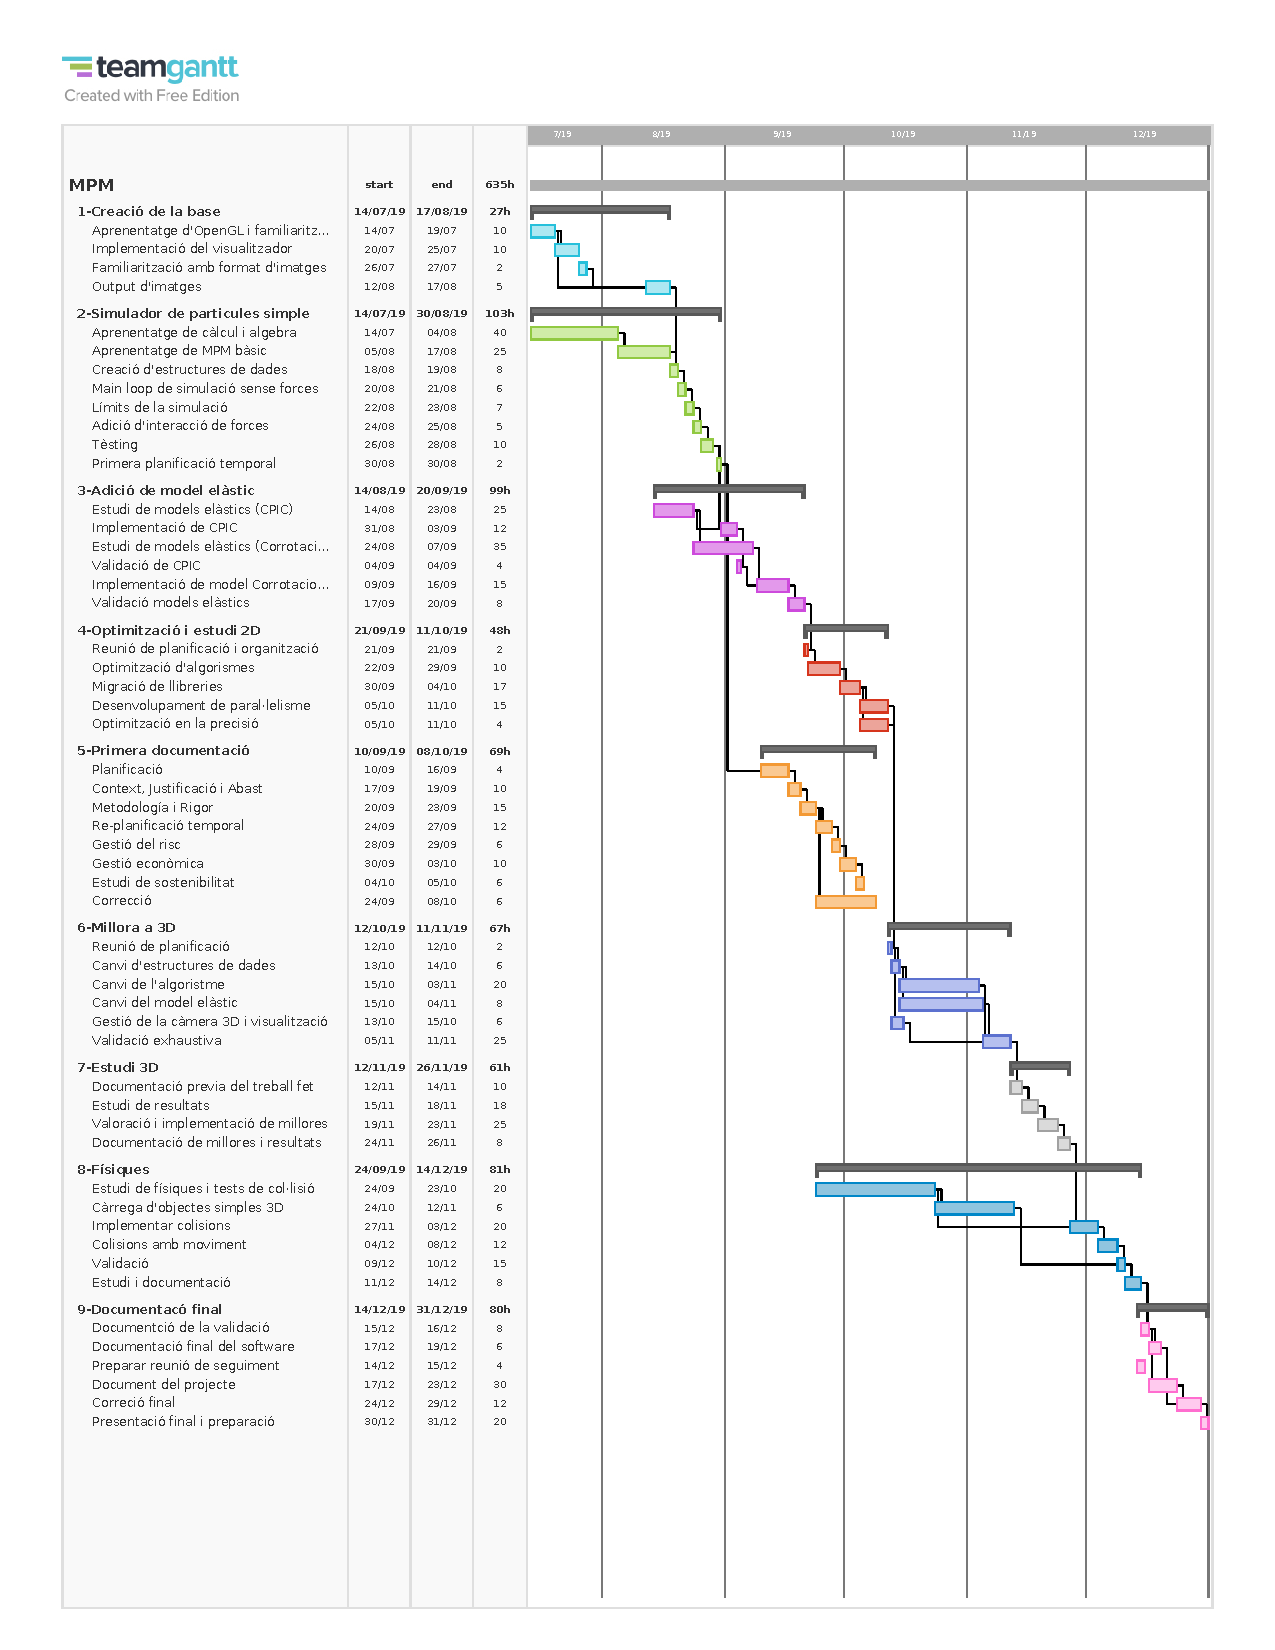
\includegraphics[width=1.45\textwidth,center]{images/Gantt.pdf}%
		\caption[\textit{Diagrama de Gantt}]{\textit{\small Diagrama de Gantt}. Creat amb \cite{Teamgantt2019}. Elaboració pròpia.}
		\label{fig:Gantt}
	\end{figure}

	\subsection{Planificació d'alternatives} \label{section:alternatives}
	En qualsevol projecte d'aquestes magnituds, tota planificació es pot esbiaixar a causa d'obstacles i inconvenients (tant directes com indirectes) que poden sorgir en qualsevol etapa, i ser de tipologies molt diverses. Tot això, en definitiva, sempre comportarà una pèrdua important de temps que cal tenir en compte. \par
	Abans de res, és important notar que les duracions estimades de les tasques estan fetes a l'alça, i atès que usem una metodologia \textit{Kanban} en acabar una tasca es començarà immediatament amb la següent. Aquest petit detall ens pot acabar proporcionant un marge de temps extra per a tractar qualsevol imprevist a sorgir.\par
	Si succeís que una tasca essencial ens importunés, seria necessari endarrerir l'entrada en escena de les consecutives etapes de manera estratègica. \par
	En qualsevol cas però, sempre s'haurà de discutir el pla d'acció amb el director del projecte durant les reunions de seguiment, i sobretot en cas d'aparèixer un problema.\par
	De ser necessari, s'eliminaran etapes del projecte, amb l'objectiu de què aquest acabi satisfactòriament a temps. \par
	Una altra opció és substituir una etapa d'implementació i estudi, per una basada a teoritzar el funcionament de quelcom d'acord amb els resultats obtinguts, sense requerir més recursos. Així podem reduir el temps d'una tasca de manera important, tot i que els resultats no seran tangibles. \par
	Particularment s'eliminaria o modificaria l'etapa número 8, ''implementació de físiques", doncs no és absolutament essencial i ens dóna, de ser necessari, fins a 80 hores de marge per a finalitzar qualsevol altra fase del projecte. Aquestes 80 hores han de ser extretes com a últim recurs, però també és important ser conscient que és un recurs existent que ens garanteix, amb molta seguretat, tenir temps suficient per a finalitzar el treball. És a dir: no es modificaria la duració del projecte. \par
	Els obstacles que ens podem trobar en aquest projecte són de dues tipologies:
	\begin{itemize}
		\item \textbf{Humans:} Problemes d'aprenentatge, a la implementació, o durant la validació que provoquen el retard de la posada en marxa de les posteriors fases. Aquests inconvenients són previsibles amb moderat temps d'antelació durant la realització, dia a dia, del treball; d'aquesta manera podem planificar un pla d'acció adequat per a mitigar el cost temporal de l'obstacle.\par
		En un projecte d'investigació, aquesta tipologia d'obstacles són molt difícils de comptabilitzar en hores, ja que durant la planificació no se sap exactament quin serà el procediment dut a terme; de totes maneres, es suposa que aquest temps a invertir de més no superarà el 10\% del temps total de la tasca.
		\item \textbf{Materials:} Les màquines s'espatllen, i quan això succeeix es poden perdre dades i, per tant, hores en reparar el hardware i a recuperar la informació. Aquest imprevist s'intentarà mitigar tenint sempre copies de seguretat del projecte, i com que es disposa de dos ordinadors, en cas que un falli s'usarà l'altre. L'impacte d'avaries de hardware serà més econòmic que temporal, especificat correctament a l'apartat \ref{section:imprevistos}.
	\end{itemize}


	\section{Gestió econòmica del projecte}
	En aquest apartat s'analitzarà l'impacte econòmic d'aquest projecte. Com que es tracta d'una activitat de recerca i investigació no hi ha costos de producció, ni de comercialització. És a dir: es tractaran els costos del disseny, planificació, estudi, implementació, recursos humans i materials de la indagació en nous coneixements. \par 
	Per a calcular el cost d'amortització, es tindrà en compte la vida útil del component en comparació amb la duració del projecte, de fins a 6 mesos en l'actual cas. \par 
	Cal afegir que s'usarà el punt com a indicador de decimals en aquest apartat, i tres xifres decimals significatives en els càlculs.
	
	\subsection{Hardware}
	Tenim en compte el cost de dos ordinadors de sobretaula, que serviran per al desenvolupament i la renderització de simulacions. En concret disposem de les següents característiques.
	\begin{itemize}
		\item \textbf{Ordinador Sobretaula:} \textit{AMD Ryzen 5 2600} 3.40GHz x 6, \textit{GeForce GTX 1060} 6GB VRAM, 16GB de RAM, 256GB SSD i 2TB HDD.
		\item \textbf{Ordinador Renderitzador:} \textit{Intel Core i7-6700} 3.40GHz x 8, \textit{GeForce GTX 1050} 4GB VRAM, 32GB RAM, 512GB SSD i 4TB HDD. Cal puntualitzar que considerem que aquest PC té una vida útil inferior a causa d'estar constantment sotmès a execucions que requereixen considerable potència de manera molt continuada.
	\end{itemize}
	Costs representats a la taula \ref{table:hardwareCosts}, comptabilitzant una mitjana de 5 hores de dedicació diàries de 220 dies laborables anuals, usant la formula \ref{eq:costs}. Per a la comptabilització de les hores, s'estima que un 65\% del treball es durà a terme amb l'ordinador de sobretaula, i el restant 35\% amb el renderitzador, sobre les 600 hores aproximades de duració del projecte. \par
	
	\begin{equation} \label{eq:costs}		\hspace*{-1cm}
		Cost  = \text{Cost equip} \cdot \frac{1 \text{ vida útil}}{4 \text{ anys} } \cdot \frac{1 \text{ any}}{220 \text{ dies lab.}} \cdot \frac{1 \text{ dia}}{5 \text{ Hores dedicacio}} \cdot \text{ Hores dedicades}
	\end{equation}
	
	\begin{table}[h!]
		\centering
		\begin{tabular}{|| c || c | c | c| c||}
			\hline
			\textbf{Producte} & \textbf{Cost} & \textbf{Vida útil} & \textbf{Hores}& \textbf{Amortització} \\
			\hline \hline
			Ordinador Sobretaula & 890.000\euro & 4 anys &390& 78.886\euro \\
			%\hline
			Ordinador Renderitzador & 1 400.000\euro & 4 anys &210& 66.818\euro \\
			\hline \hline
			\textbf{Total} & - & - & 600 & 145.704\euro \\
			\hline
		\end{tabular}
		\caption[\textit{Costs Hardware}]{\textit{\small Costs Hardware}. Elaboració pròpia}
		\label{table:hardwareCosts}
	\end{table}

	\subsection{Software}
	Per aquest projecte, s'ha usat un cert nombre de programes de pagament, i altres de gratuïts o \textit{Open Source}. Els productes de pagament, han sigut obtinguts de manera gratuïta gràcies a llicències d'estudiants oferides per la FIB.
	Queden recollits en la taula \ref{table:softwareCosts}, a continuació.
	\begin{table}[h!]
		\centering
		\begin{tabular}{|| c || c | c||}
			\hline
			\textbf{Producte} & \textbf{Preu} &\textbf{Amortització} \\
			\hline \hline
			Git		 	& 0.000\euro 	& 0.000\euro \\
			GitKraken\footnote	& 48.000\euro   & 0.000\euro \\
			\LaTeX 		& 0.000\euro 	& 0.000\euro \\
			TeamGantt 	& 0.000\euro	& 0.000\euro \\
			Ubuntu OS 	& 0.000\euro  	& 0.000\euro \\
			Visual Studio 2019\footnote& 641.000\euro & 0.000\euro \\
			Windows 10\footnote[3] 	& 145.000\euro 	& 0.000\euro \\
			\hline \hline
			\textbf{Total} & 834.000\euro & 0.00\euro \\
			\hline
		\end{tabular}
		\caption[\textit{Costs Software}]{\textit{\small Costs Software}. Elaboració pròpia}
		\label{table:softwareCosts}
	\end{table}
		\footnotetext[2]{Obtingut amb la llicència de \textit{GitHub Student Pack}}
		\footnotetext[3]{Obtingut amb la llicència de \textit{Windows Azure Education}}
	
	\subsection{Recursos Humans}
	Els costs de recursos humans fan referència a les diverses funcions que realitza, en aquest cas, l'únic treballador que realitza el projecte. S'ha decidit excloure del pressupost al director del projecte, ja que s'ha considerat que és tracta d'un cost de consultoria i suport gratuïts per part de la universitat.
	\par 
	En aquest cas el treballador farà les funcions de coordinador, analista, desenvolupador i tester (conegut com a \textit{Test engineer}); i la seva dedicació en hores, així com el cost associat  en cadascuna de les seves respectives tasques, es troba en les taules \ref{table:humansCost} i \ref{table:taskCost}. \par
	Els costs són estimats suposant treballadors assalariats, acollint-nos a una jornada laboral màxima de 1800 hores anuals, d'acord amb el BOE 2016-2856\cite{boe}, i seleccionant els sous de la web \textit{Indeed}\cite{indeed} com a referents per als següents càlculs\footnote{Basats en la mitjana americana, d'una població de com a mínim 3500 individus.}. Per a calcular el cost amb la despesa de Seguretat Social, s'adjunta aquesta quantitat comptabilitzada com el 35 per cent del sou brut.
	\begin{table}[h!]
		\centering
		\hspace*{-1cm}
		\begin{tabular}{|| c || c | c | c | c ||}
			\hline
			\textbf{Posició} & \textbf{Salari brut (\euro/hora)} & \textbf{Hores} & \textbf{Cost} & \textbf{+ Seguretat Social}\\
			\hline \hline
			Coordinador	& 23.773	& 137	& 3 256.901\euro	& 4 396.816\euro \\
			Analista	& 33.673	& 50	& 1 683.650\euro	& 2 272.927\euro \\
			Desenvolupador &	46.943 & 358	& 16 805.594\euro	& 22 687.551\euro \\
			Tester 		&	50.799 & 68 & 3 454.332\euro	& 4 663.348\euro \\			
			\hline \hline 
			Total & - & 613 & 25 200.477\euro & 34 020.644\euro \\ 
			\hline
		\end{tabular}
		\caption[\textit{Cost RRHH}]{\textit{\small Cost Recursos Humans}. Elaboració pròpia.}
		\label{table:humansCost}
	\end{table}

	\begin{table}[h!]
		\centering
		\begin{tabular}{|| c | c || c | c | c ||}
			\hline
			\textbf{Id} & \textbf{Activitat} & \textbf{Hores} & \textbf{RRHH} & \textbf{Cost (\euro)} \\
			\hline
			0 & Total & 613 & - & 25 200.477\euro \\ % 24 915.328
			\hline \hline
			1 & Creació de la base & 25 & Desenvolupador & 1 173.575\euro \\
			\hline \hline
			2 & Simulador de partícules simple & 100 & - & 4 732.860\euro\\
			\hline
			2.1 & Aprenentatge \textit{solver} & 65 & Desenvolupador &  3 051.295\euro \\
			2.2 & Implementació \textit{solver} & 25 & Desenvolupador & 1 173.575\euro \\
			2.3 & Validació \textit{solver} & 10 & Tester & 507.990\euro \\
			\hline \hline
			3 & Addició model elàstic & 98 & - & 4 631.209\euro \\
			\hline
			3.1 & Aprenentatge models elàstics & 60 & Desenvolupador & 2 816.580\euro \\
			3.2 & Implementació models elàstics & 30 & Desenvolupador & 1 408.290\euro \\
			3.3 & Validació models elàstics & 8 & Tester & 406.339\euro \\
			\hline \hline
			4 & Optimització i estudi 2D & 45 & - & 1 714.335\euro \\
			\hline
			4.1 & Estudi 2D & 30 & Analista & 1 010.190\euro \\ 
			4.2 & Paral·lelisme & 15 & Desenvolupador & 704.145\euro \\
			\hline \hline
			5 & Primera documentació & 65 & - & 1 545.245\euro \\ 
			\hline
			5.1 & Documentació: planificació & 20 & Coordinador & 475.46\euro \\ 
			5.2 & Documentació: redacció & 35 & Coordinador & 832.055\euro \\
			5.3 & Documentació: correcció & 10 & Coordinador & 237.730\euro \\
			\hline \hline
			6 & Millora a 3D & 60 & -& 2932.260\euro \\
			\hline
			6.1 & 3D: migració & 30 & Desenvolupador & 1 408.290\euro \\
			6.2 & 3D: validació & 30 & Tester & 1 523.970 \euro \\
			\hline \hline
			7 & Estudi i recerca 3D & 60 & - & 2 319.48\euro \\
			\hline
			7.1 & Estudi 3D & 20 & Analista & 673.46\euro \\ 
			7.2 & Documentació 3D & 10 & Coordinador & 237.730\euro \\
			7.3 & Estudi3D: millores i validació & 30 & Desenvolupador & 1 408.290\euro \\
			\hline \hline
			8 & Físiques & 80 &  - & 3 832.560\euro \\
			\hline
			8.1 & Aprenentatge físiques & 20 & Desenvolupador & 938.860\euro \\
			8.2 & Implementació físiques & 30 & Desenvolupador & 1 408.290\euro \\
			8.3 & Validació físiques & 20 & Tester & 1 015.980\euro \\
			8.4 & Implementació eines & 10 & Desenvolupador & 469.430\euro \\
			\hline \hline
			9 & Documentació final & 80 & - & 1 901.840\euro \\
			\hline
			9.1 & Documentació programa & 18 & Desenvolupador & 844.974\euro \\
			9.2 & Redacció memòria & 30 & Coordinador & 713.190\euro \\
			9.3 & Revisió i correcció & 12 & Coordinador & 285.276\euro \\
			9.4 & Preparació i defensa final & 20 & Coordinador & 475.460\euro \\
			\hline
		\end{tabular}
		\caption[\textit{Cost RRHH per tasca}]{\textit{\small Cost recursos humans per tasca}. Elaboració pròpia.}
		\label{table:taskCost}		
	\end{table}

	\subsection{Imprevistos}\label{section:imprevistos}
	En cas d'esdeveniments inesperats en el desenvolupament del projecte, una part del pressupost s'ha destinat, per totes les posicions corresponents a recursos humans, a tenir en compte hores extra com a cost addicional. Veure taula \ref{table:imprevistosRH}.
	\begin{table}[h!]
		\hspace*{-.5cm}
		\centering
		\begin{tabular}{|| c || c | c || c | c||}
			\hline
			\textbf{Posició} & \textbf{Hores} & \textbf{Cost + SS (\euro)} & \textbf{Probabilitat} & \textbf{Imputació (\euro)} \\
			\hline \hline
			Coordinador & 10 & 320.936\euro & 30\% & 96.291\euro \\
			Analista & 5 & 227.293\euro & 5\% & 11.365\euro \\
			Desenvolupador & 20 & 1 267.461\euro & 40\% & 506.984\euro\\
			Tester & 10 &  685.787\euro & 8\% & 54.863\euro \\
			\hline \hline
			Total & 45 & 2 501.477\euro & - & 669.503\euro \\
			\hline
		\end{tabular}
		\caption[\textit{Imprevistos RRHH}]{\textit{\small Imprevistos recursos humans}. Elaboració pròpia}
		\label{table:imprevistosRH}
	\end{table}

	La distribució d'hores addicionals es fa tenint en compte la magnitud de l'impacte esperat de qualsevol error produït per cadascuna de les posicions, i el temps a dedicar en el projecte. Com que el treball usa una metodologia molt ''ràpida" \text{ i} l'assignació d'hores és prou laxa, i no s'esperen imprevists importants en les àrees de validació i anàlisi; però existeix una probabilitat elevada del fet que la implementació i organització del projecte s'allarguin en succeir algun error comú d'aquestes temàtiques.
	\par 
	A més a més, cal afegir una partida per a imprevists materials, avaries, o altres problemes que poden sorgir de manera circumstancial i aliena als mateixos recursos humans. Aquest pressupost es pot veure  a la taula \ref{table:imprevistosM}.
	\begin{table}[h!]
		\centering
		\begin{tabular}{|| c || c | c || c | c ||}
			\hline
			\textbf{Recurs} & \textbf{Imprevist} & \textbf{Cost (\euro)} & \textbf{Probabilitat} & \textbf{Imputació (\euro)} \\
			\hline\hline
			\multirow{3}{*}{Ordinador} & 
					Falla de disc & 80\euro & 5\% & 4.000\euro \\
					&RAM malmesa  &  50\euro & 3\% & 1.500\euro \\
					&Servei de reparació 	 & 60\euro & 10\% & 6.000\euro \\
			\hline 
			Perifèrics & Avaria & 25\euro & 5\% & 1.250\euro\\
			\hline
			Material & Substitució & 10\euro & 50\% & 5.000\euro \\
			\hline \hline
			Total & - & 225\euro & - & 17.750\euro\\
			\hline
		\end{tabular}
		\caption[\textit{Imprevistos materials}]{\textit{\small Imprevistos materials}. Elaboració pròpia}
		\label{table:imprevistosM}
	\end{table}
	
	\subsection{Costs indirectes} \label{section:cIndirectes}
	Els costs indirectes, donat que no són calculables precisament, s'intenten aproximar el millor possible en aquest apartat. \par
	Pel que fa als costs elèctrics, es comptabilitza el preu per quilowatt hora a 0.11 \euro/kWh, i s'ha calculat un consum mitjà de l'ordinador de sobretaula de 240 Watt. Com que aquest terminal s'usarà, aproximadament, 500 hores, podem calcular l'energia consumida com a 120 kW, o 13.2\euro. \par
	Per altra banda, disposem de l'ordinador per a computar els tests. Aquest, tot i que s'usarà una mitjana de 70 hores, té un consum molt més elevat que l'ordinador de sobretaula, ja que estarà treballant a màxima potència tota l'estona. Aquest fet ens dóna una potència esperada de 600 Watt, el que ens equival a una energia consumida de 42 kWh, o 4.62 \euro \par
	També podem sumar el cost elèctric dels perifèrics, com les pantalles, amb un consum equivalent a 28 Watts durant 530 hores; és a dir: 14.84 kWh o 1.632\euro. \par
	Afegim també els costs de transport per anar al CRV, on se situa el laboratori del ViRVIG, que es correspon amb viatges durant 3 mesos i es comptabilitzen amb els seus respectius descomptes, equivalent a 52.5\euro en total. \par
	I finalment cobrim els costs de connexió a la xarxa, segons l'import mensual de 36.99\euro, durant els 6 mesos de duració del projecte, equivalent en definitiva 221.94\euro.\par
	A la taula \ref{table:imprevistosI} podem observar un resum.
	\begin{table}[h!]
		\centering
		\begin{tabular}{||c|| c||}
			\hline
			\textbf{Font} & \textbf{Cost(\euro)} \\
			\hline \hline
			Ordinador sobretaula & 13.200\euro \\
			Ordinador rendering & 4.620\euro \\
			Perifèrics & 1.632\euro \\
			Transport & 52.500\euro \\
			Connexió a internet & 221.940\euro\\
			\hline \hline
			Total & 293.892\euro\\
			\hline
		\end{tabular}
		\caption[\textit{Costs Indirectes}]{\textit{\small Costs Indirectes}. Elaboració pròpia}
		\label{table:imprevistosI}
	\end{table}
	
	
	\subsection{Contingència}
	Reservem una part dels diners, per a qualsevol altre imprevist dels ja anomenats; garantint així la correcta realització del projecte sense inconvenients monetaris. Per a això reservarem uns diferents percentatges depenent de l'origen del cost, i el seu objectiu. Podem veure el pressupost de contingència a la taula \ref{table:contingencia}.
	
	\begin{table}[h!]
		\centering
		\begin{tabular}{|| c || c | c | c |}
			\hline
			\textbf{Font} & \textbf{Preu(\euro)} & \textbf{Percentatge} & \textbf{Cost(\euro)} \\
			\hline \hline
			Recursos Humans & 34 020.644\euro & 2\% & 680.413\euro \\
			\hline
			Imprevistos & 225.000\euro & 15\% & 33.750\euro \\
			\hline
			Costs indirectes & 293.892\euro & 15\% & 44.084\euro \\
			\hline \hline
			Total & - & - & 758.247\euro \\
			\hline
		\end{tabular}
		\caption[\textit{Pla de contingència}]{\textit{\small Pla de contingència}. Elaboració pròpia}
		\label{table:contingencia}
	\end{table}

	S'assigna un 10\% de contingència a recursos humans, ja que aquest pressupost ja té en compte imprevistos temporals, i per tant l'impacte serà menor. Per altra banda situem la contingència de la resta d'imprevistos i dels costs indirectes del projecte a un 15\% per a cobrir qualsevol mancança en aquest aspecte.
	
	\subsection{Pressupost final}
	Finalment, reunim en la següent taula \ref{table:pressupostFinal} el sumatori de totes les partides del pressupost, per a obtenir una visió general del cost del projecte i la distribució de la inversió en aquest.
	
	\begin{table}[h!]
		\centering
		\begin{tabular}{|| c | c ||}
			\hline
			\textbf{Font} & \textbf{Cost(\euro)} \\
			\hline \hline
			Hardware & 145.704\euro \\
			Software & 0.000\euro \\
			Recursos Humans & 34 020.644\euro \\
			Imprevistos RRHH & 669.503\euro \\
			Imprevistos materials & 17.750\euro \\
			Costs indirectes & 293.892\euro \\
			Contingència  & 758.247\euro \\
			\hline \hline
			Total & 35 905.740\euro \\
			\hline
		\end{tabular}
		\caption[\textit{Pressupost final}]{\textit{\small Pressupost final}. Elaboració pròpia}
		\label{table:pressupostFinal}
	\end{table}
	Les partides de contingència, imprevistos de recursos humans i materials, en cas de no ser consumides seran reservades per a futurs projectes; de manera que els diners seguiran sent destinats a la investigació i usats apropiadament.
	
	\subsection{Control de gestió}
	Per a gestionar correctament el pressupost al llarg del desenvolupament del projecte, s'ha seleccionat una sèrie d'indicadors per a poder seguir, i tenir en compte, l'evolució del projecte i la diferència entre el cost real i estimat a escala de tasca. Per detectar desviacions en el pressupost s'usaran les següents fórmules a tall d'indicadors:
	\begin{equation*}
	\begin{split}
		\text{Desviació del Cost } &= (C_e-C_r) \cdot T_r \\ 
		\text{Desviació Eficiència } &= (T_e - T_r) \cdot C_e 
	\end{split}
	\end{equation*}
	On $C$ correspon al cost en $\frac{\text{\euro}}{hora}$, i $T$ correspon al temps en hores. Els subíndexs $r$ i $e$ senyalen la realitat o l'estimació, respectivament. \par
	Aquests indicadors ens poden ajudar a mesurar les desviacions, sobretot, a les partides de recursos humans per tasca, doncs són les més impactants al projecte.
	
	\subsection{Viabilitat econòmica} \label{section:viabilitat}
	Aquest projecte és d'investigació, recerca i divulgació; i per tant no es cerca obtenir beneficis. D'aquesta manera, la viabilitat econòmica depèn de les subvencions i ajuts rebuts per part dels contribuents, que fan possible la realització de molts projectes d'aquesta temàtica i que segueixen la mateixa noció. \par
	De totes maneres, la viabilitat econòmica va estrictament lligada a un control ajustat del pressupost, seguint uns certs procediments al final de cadascuna de les tasques a realitzar. L'objectiu d'aquest seguiment és calcular la diferència entre el cost esperat i el real, detectar desviacions en el pressupost i corregir-les com més aviat millor. \par
	Les correccions a aplicar per assegurar la viabilitat econòmica han sigut descrites anteriorment, a la secció \ref{section:alternatives}, es basen a cobrir costs inesperats, replanificar etapes i retallar tasques.
	
	\section{Informe de Sostenibilitat}
	La sostenibilitat no és una qüestió en la qual es pensi activament ni de bon tros, però és inherent a qualsevol activitat que es du a terme, concepte, producte, formació... i particularment en tot el que involucra recursos TIC, que en l'era de la informació són omnipresents. \par
	Trobo essencial tenir intenció; intenció d'aprendre i millorar el nostre entorn, intenció de ser crític, i intenció de fer les coses bé. Pot ser que un mai hagi estat instruït en tècniques, conceptes, o indicadors de sostenibilitat; però si es té intenció de valorar i enriquir el tarannà de si mateix, molt errat no es pot anar. Amb això vull dir que no és necessari ser un expert per a poder aportar quelcom a l'entorn i la societat, i a ajudar al fet que aquesta sigui més sostenible. \par
	Aquesta intenció també demostra un interès actiu i una consciència de l'impacte que un mateix pot arribar a tenir, reflectida en no només el ''què" es fa, sinó amb el ''com" es fa. Aquesta és la meva mentalitat al dur a terme aquest projecte. \par
	La comprensió del poder que es té amb els recursos TIC ens atorga la capacitat, inevitablement, d'afectar en major o menor mesura el nostre entorn i, per tant, si busquem un àmbit més sostenible, estarem maximitzant l'impacte positiu de la nostra activitat professional sobre la societat. \par
	Com a reflexió cal dir que és necessari tenir intenció, però no és suficient; trobo que a vegades cal anar més enllà, ser crític amb un mateix, i intentar millorar el que ja s'ha fet, cercar informació i aprendre per a fer una millor feina, i ser més sostenible. Un exemple clar seria l'aprenentatge i comprensió d'indicadors de les tres dimensions de la sostenibilitat, que ajuden a la correcta mesura i apreciació del potencial impacte del projecte. \par
	Aquest fet es transmet a escala personal, tot i sempre intentar dur a terme les coses de manera correcta, he de reconèixer que mesurar a l'hora de la veritat la potencial empremta del projecte és una tasca desconeguda per a mi, així com el control de la dimensió econòmica i el coneixement d'indicadors de sostenibilitat. Per això parlo d'intenció, perquè espero millorar en aquest aspecte, i aconseguir elevar el treball a un següent nivell.
	
	\subsection{Dimensions de la sostenibilitat}
	\subsubsection{Dimensió econòmica}
	Com s'ha mencionat anteriorment a la secció \ref{section:viabilitat}, el projecte té un cost econòmic estimat de 35 905.740\euro. Tot i això, la viabilitat econòmica del projecte posat en producció no és valorable en beneficis monetaris, doncs aquests no es produiran. La motivació del projecte, a més de personal, busca millorar les solucions existents, i conseqüentment ha d'animar a altres investigadors a millorar l'estat actual de \textit{MPM} i dur a terme millores progressives; fet que provocarà l'aparició de nous projectes mentre aquest sigui una solució acceptable i potent. \par
	És un projecte de recerca i investigació amb un cost moderadament elevat, a causa de l'amplitud de coneixements a incorporar i a validar, però en futurs projectes aquest cost serà amortitzat, ja que aquests coneixements ja estaran adquirits. \par
	En aquest projecte, concretament, busquem una solució més eficient que permeti simular més ràpidament un entorn concret, i sense necessitar un gran nombre de recursos; disminuint el desgast de components d'un processador, i reduint el cost econòmic de temps de simulació necessaris.
	
	\subsubsection{Dimensió ambiental}
	Els costos ambientals durant la realització del projecte, poden ser mesurats amb les dades obtingudes a la secció \ref{section:cIndirectes} en quilowatts hora consumits, d'un total de 176.67kWh de consum energètic durant l'etapa del projecte posat en producció (PPP). Caldria comptabilitzar, a més a més, les emissions de CO$_{2}$ produïdes pel transport públic usat per a viatjar al ViRVIG, i produïdes per generar l'electricitat consumida. \par
	En el pitjor dels supòsits, en que la totalitat de l'electricitat prové d'una planta de crema de carbó, podem calcular una producció de 0.94Kg de CO$_2$ per cada quilowatt hora consumit; és a dir: 166.067Kg de CO$_2$ produïts pel projecte. Pel que fa al transport, sempre s'ha viatjat en tren o autobús, i s'ha calculat una aproximació 8.16Kg de CO$_2$ produït per aquest, donada una producció de 0.98 grams de CO$_2$ per quilòmetre. Per tant, hem generat una petjada de carboni equivalent a 174.227Kg de CO$_2$. \par
	Pel que fa a la vida útil del projecte, des d'un punt de vista ambiental pot aportar una millora, ja que aquest busca reduir, i minimitzar, el temps i l'energia requerida per a efectuar certes simulacions. Això recau en un consum elèctric menor, i per tant una menor petjada de carboni respecte a les solucions existents actualment. \par
	Pel que fa a riscs de caràcter ambiental, aquest projecte no en provoca de cap classe. En el pitjor dels casos, no es produiria cap millora, i ens quedaríem en l'estat previ a l'inici del projecte; i en el millor dels casos, haurem millorat les solucions existents de manera més sostenible.
	
	\subsubsection{Dimensió social}
	Aquest projecte ha proporcionat a l'autor una àmplia base en simulació de fluids, així com en disciplines molt diferenciades de la branca cànon de la informàtica. L'aprenentatge d'aquesta temàtica ha sorgit d'un interès personal, el qual es demostrarà útil i una experiència productiva per a futurs projectes de tota mena, així com estimular la reusabilitat del mateix treball per a aprofundir més en aquest. \par
	En l'àmbit social, aquest projecte és difícil que millori de manera significativa l'estat de l'art actual dels simuladors de fluids; però sí que busca ser un punt de partida i introducció en aquest extens i difícil camp, ja que existeixen pocs documents a la literatura, o a la comunitat, que puguin ser usats per quelcom amb l'objectiu d'introduir-se en la simulació de fluids, d'aquesta manera s'espera que aquesta memòria pugui servir per a suplir aquesta mancança. \par
	Si aquest últim punt és ben aprofitat, les possibilitats són molt altes que s'usi aquest treball com a base per a que altres estudiants puguin reproduir els resultats aquí descrits, i aprofundir en altres subcamps de la simulació de fluids. \par
	En contrast, la possibilitat que el projecte tingui un impacte negatiu a la societat és molt baixa, i depèn de la qualitat del treball per a servir de guia futura a altres alumnes, o persones que vulguin aprendre sobre aquesta temàtica.
	
	\subsection{Matriu de sostenibilitat}
	A manera de resum, presentem la següent matriu de sostenibilitat representada a la taula \ref{table:sustanMatrix} per a sintetitzar els anteriors apartats.
	
	\begin{table}[h!]
		\centering
		\hspace*{-1cm}
		\begin{tabular}{|| c || c | c | c ||}
			\hline
			& \textbf{PPP} & \textbf{Vida útil} & \textbf{Riscs} \\
			\hline \hline
			\textbf{Econòmica} & 38 917.670\euro & No beneficis & La no viabilitat econòmica \\
			\hline
			\textbf{Ambiental} & 174.227KgCO$_2$ & Reducció energètica &La no millora \\
			\hline
			\textbf{Social} & 9/10 & 7/10 & Pocs \\ 
			\hline
		\end{tabular}
		
		\caption[\textit{Matriu de sostenibilitat}]{\textit{\small Matriu de sostenibilitat}. Elaboració pròpia.}
		\label{table:sustanMatrix}
	\end{table}
	
	% REFERENCIES
	\newpage
	
	\renewcommand{\bibname}{Referències}
	
	\bibliography{BibTex/cit} 
	\bibliographystyle{ieeetr}
	
	%\newpage
	
	%\renewcommand\listfigurename{Llistat d'imatges}
	%\listoffigures
	%\listoftables
	
\end{document}